\documentclass[a4paper, 12pt]{article}
\usepackage[brazil]{babel}
\usepackage[utf8x]{inputenc}
\usepackage{amsmath, amssymb, exscale}
\usepackage{enumerate}
\usepackage{amsfonts}
\usepackage{graphicx, graphics}
\usepackage[colorinlistoftodos]{todonotes}
\usepackage{texnames}
\usepackage{geometry}
\usepackage{booktabs}
\usepackage{float}
\usepackage{icomma}
\usepackage{longtable}
\usepackage[pdftex]{hyperref}
\usepackage{subfigure}
\usepackage[hang]{caption}
\usepackage[american, siunitx]{circuitikz}
\usetikzlibrary{arrows,shapes,calc,positioning}
\usepackage{comment}
\usepackage{cite}
\usepackage{setspace} 
\usepackage{array}
\usepackage{siunitx}
\usepackage{leading}
\usepackage{indentfirst} %Permite a utilização de marcadores
\usepackage{titlesec} %Formata as seções com o pacote
\usepackage{parskip}
\usepackage{quoting}
\usepackage{multicol}
\usepackage{epstopdf}

\setlength{\captionmargin}{12 pt}
\DeclareCaptionLabelSeparator*{tab}{\linebreak}
\captionsetup{labelsep = endash}
\addto\captionsbrazil
{
\renewcommand{\figurename}{FIGURA}
\renewcommand{\tablename}{TABELA}
}

\DeclareMathOperator{\sen}{sen}
\renewcommand{\sin}{\sen}

\mathchardef\comma=\mathcode`.
\DeclareMathSymbol{.}{\mathord}{letters}{"3B}

\geometry{hmargin = {3 cm, 2 cm}, vmargin = {3 cm, 2 cm}}
\parindent = 1.5 cm 
\title{Relatório de Eletrônica I}
\author{Alvarenga}

%#########################################%

\begin{document}
\begin{titlepage}

\newcommand{\HRule}{\rule{\linewidth}{0.0mm}} 
\center 
\textsc{\Large Centro Federal de Educação Tecnológica de Minas Gerais}\\[0.7 cm]
\vskip -0.5 cm
\textsc{\Large Graduação em Engenharia Mecatrônica}\\[0.7 cm]
\vskip -0.5 cm
\textsc{\Large Campus Divinópolis}\\[0.7 cm]
\vskip -0.5 cm
\textsc{\Large Dinâmica Veicular}\\[7 cm]


\begin{center}
\textsc{\Huge Manobra Sweep Sine: \\
\large{ISO 7401}}
\\[0.5cm]
\vskip-0.2 cm
{\LARGE }\\[1 cm]

 \end{center}

\vskip 1.5 cm
\begin{center} \Large
Por:\\[1.5 cm]
Bernardo Bresolini\\
Ester Q. Alvarenga \\
Patrícia Pereira\\
Thalles O. Campagnani \\

Graduandos em Eng. Mecatrônica\\[2.5 cm]
Divinópolis-MG\\2019
\end{center}

\end{titlepage}

\tableofcontents
\pagebreak

\section{Introdução}
Dada a enorme complexidade das interações dinâmicas entre o veículo-motorista-ambiente e suas vicissitudes, é impreciso a averiguação da resposta do veículo apenas por métodos analíticos. Deve-se assim, realizar variados testes sob diversas condições, a fim de adquirir os dados necessários para uma avaliação real do comportamento veicular. Portanto, a padronização de testes que obtenham dados aos quais seja possível avaliar a resposta do carro e estabelecer critérios mínimos normalizados.

Sendo assim, o presente trabalho abordará um dos métodos padronizados pela Organização Internacional de Padronização (International Organization for Stardardization --- ISO): o sweep sine ISO 7401. De fato, a norma ISO 7401 elabora um procedimento mais abrangente do que a manobra a ser verificada, tendo o objetivo de fornecer um método capaz de fornecer resultados repetitivos e discriminatórios.

Ainda, pretende-se avaliar essa manobra em um projeto de um veículo desenvolvido pelos autores, o carro Hórus nas condições de carga mínima e máxima definidos na norma. 

\section{Sweep Sine}
A \textit{sweep sine} (seno varrente) é definida como uma função senoidal com frequência aumentando com o passar o tempo, como mostra a FIG.  \ref{graf:sweep_sine_exemplo}. Deste modo, é possível excitar um sistema nas diversas faixas de frequência de interesse. Assim, é possível obter as características de resposta em frequência: as frequências de ressonância, defasagem do sinal, ganho de amplitude.
\begin{figure}[h]
    \centering
    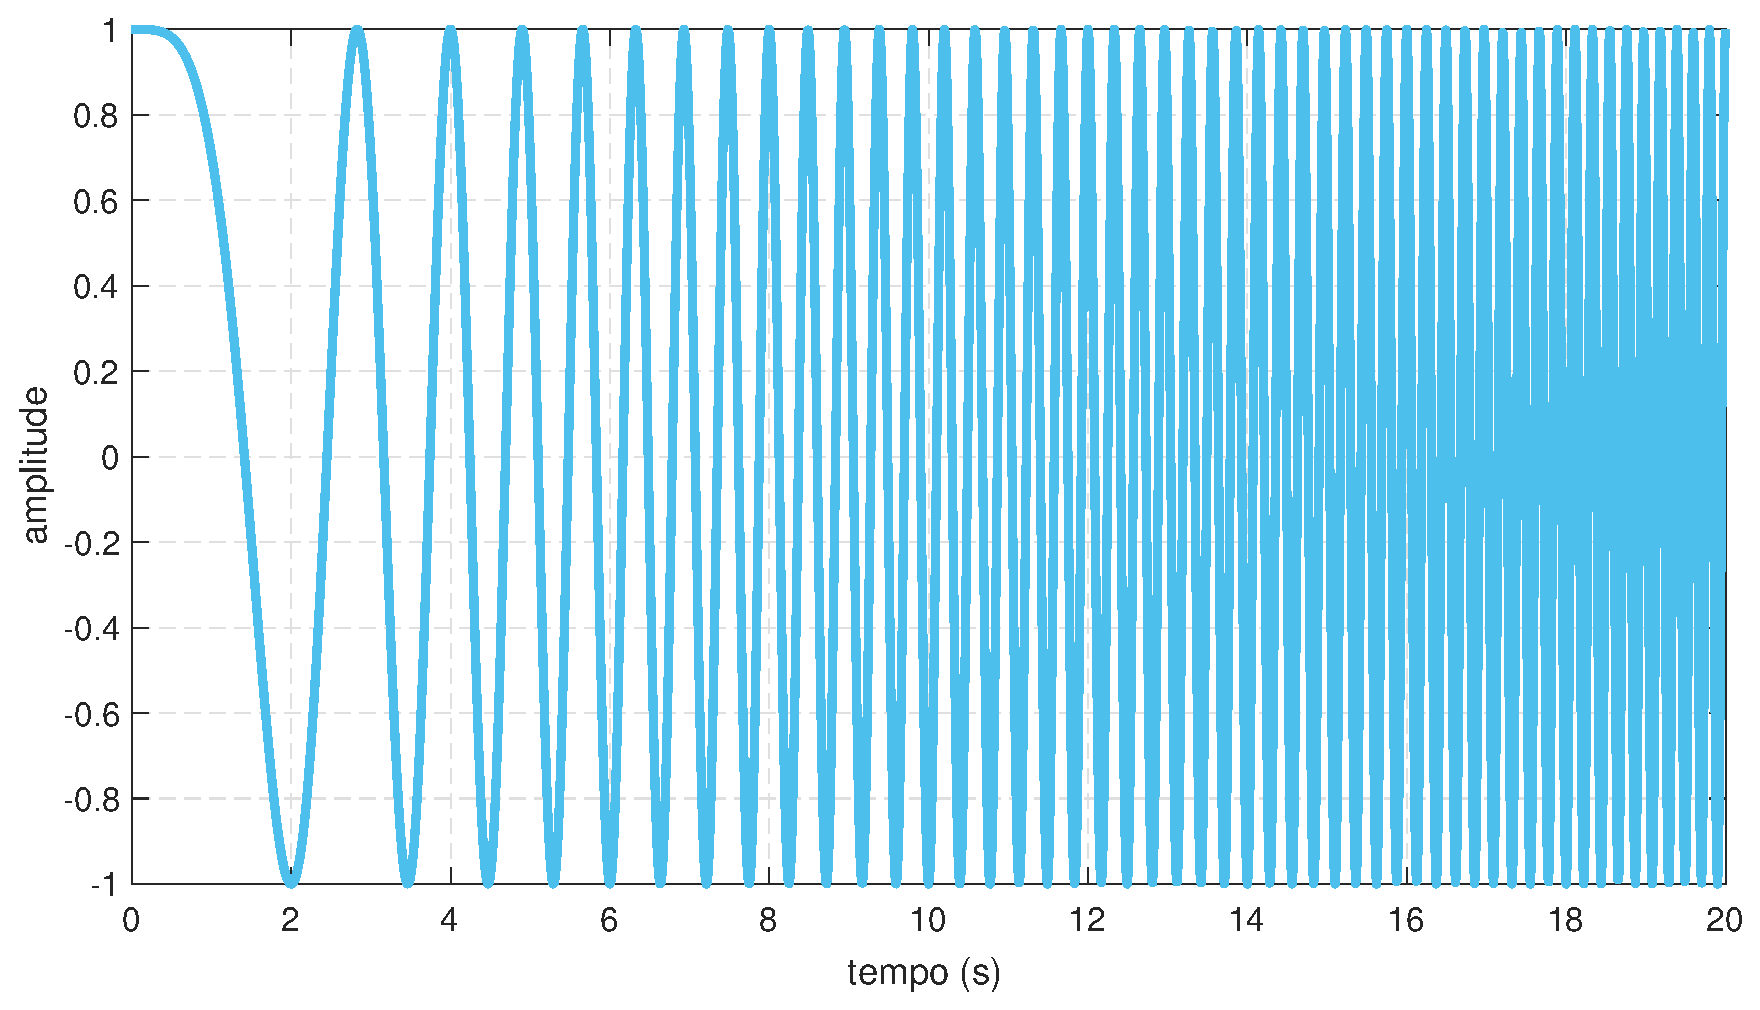
\includegraphics[width=10cm]{imagens/sweep_sine.eps}
    \caption{Demonstrativo da função \textit{sweep sine}, iniciando em 0 Hz e terminando em 5 Hz}
    \label{graf:sweep_sine_exemplo}
\end{figure}


No método descrito pela ISO 7401 (2003), as características importantes a serem obtidas é
\begin{enumerate}
    \item Velocidade lateral relacionada ao ângulo do volante;
    \item Velocidade \textit{yaw} relacionada ao ângulo do volante.
\end{enumerate}

Para tanto, é recomendável fazer os testes a 100 km/h ou em alguma velocidade desejável múltipla de 20 km/h. Dada a intenção de que o veículo transite em vias urbanas, fará-se os testes em: 100 km/h e 40 km/h.

\section{Condições de Teste}
Para que o comportamento veicular --- dada a manobra \textit{Sweep Sine} em um veículo padronizado ou não --- possa ser avaliada, é preciso estabelecer algumas condições de teste, as quais estipularão os critérios que deverão ser seguidos.

Estes critérios são estabelecidos também pela ISO 7401, que afirma que  os ensaios devem ser realizados na condição mínima de carga e na condição máxima de carga definida. A condição de carga mínima considera o peso do carro com o motorista mais a instrumentação, sendo que o peso do motorista mais o peso da instrumentação não poderão exceder 150 kg. Já a condição de carga máxima, a qual não poderá ser excedida, leva em conta o peso do carro mais o peso dos passageiros --- em que é definido o peso de 68 kg para cada passageiro --- e também o peso do bagageiro.


É também definido a velocidade de teste. Esta é estabelecida como sendo o valor nominal da velocidade longitudinal. A velocidade padrão de teste é 100 km/h. Outras velocidades de teste de interesse podem ser usadas (de preferência em etapas com diferenças de 20 km/h).

\section{Hórus}

Hórus é um veículo particular para consumidores da classe trabalhadora, com foco em uso urbano, segurança e conforto. O projeto conceitual e os requisitos do carro, optou-se por definir os seus moldes gerais como:
\begin{itemize}
    \item Compact Sedan
    \item Tração 4 × 2;
    \item 5 lugares: 2 nos bancos dianteiros e 3 nos bancos traseiros;
    \item 4 portas;
    \item Peso de 922 kg;
    \item Porta malas de 510 L;
    \item Custo por volta de R\$ 55.000,00;
    \item Ciclo de vida de 5 anos.
\end{itemize}


\section{Resultados}

Para avaliar a manobra padronizada \textit{Sweep Sine}, utilizou-se o carro em desenvolvimento Hórus e o software Adams Car. Definiu-se como velocidades longitudinais 40 km/h e 100 km/h. E as cargas máxima e mínima foram calculadas como:

\begin{align}
\mathrm{carga}_{min} &= (922 \: \textup{(hórus)} + 68 \: \textup{(Motorista)} + 10 \: \textup{(instrumentação)} ) \: \textup{kg} = 1000 \: \textup{kg} \\ 
\mathrm{carga}_{max} &= (1000 + 4\times 68 \: \textup{(passageiros)} + 228 \textup{(bagageiro)}) \: \textup{kg} = 1500 \: \textup{kg}
\end{align}

A curva de entrada para os testes a 40 km/h é dada pelo gráfico apresentado na FIG. \ref{fig:entrada40}, cuja amplitude é de 90\si{\degree}, com frequência inicial de 0,001 Hz e final de 2 Hz.
\begin{figure}[H]
\centering
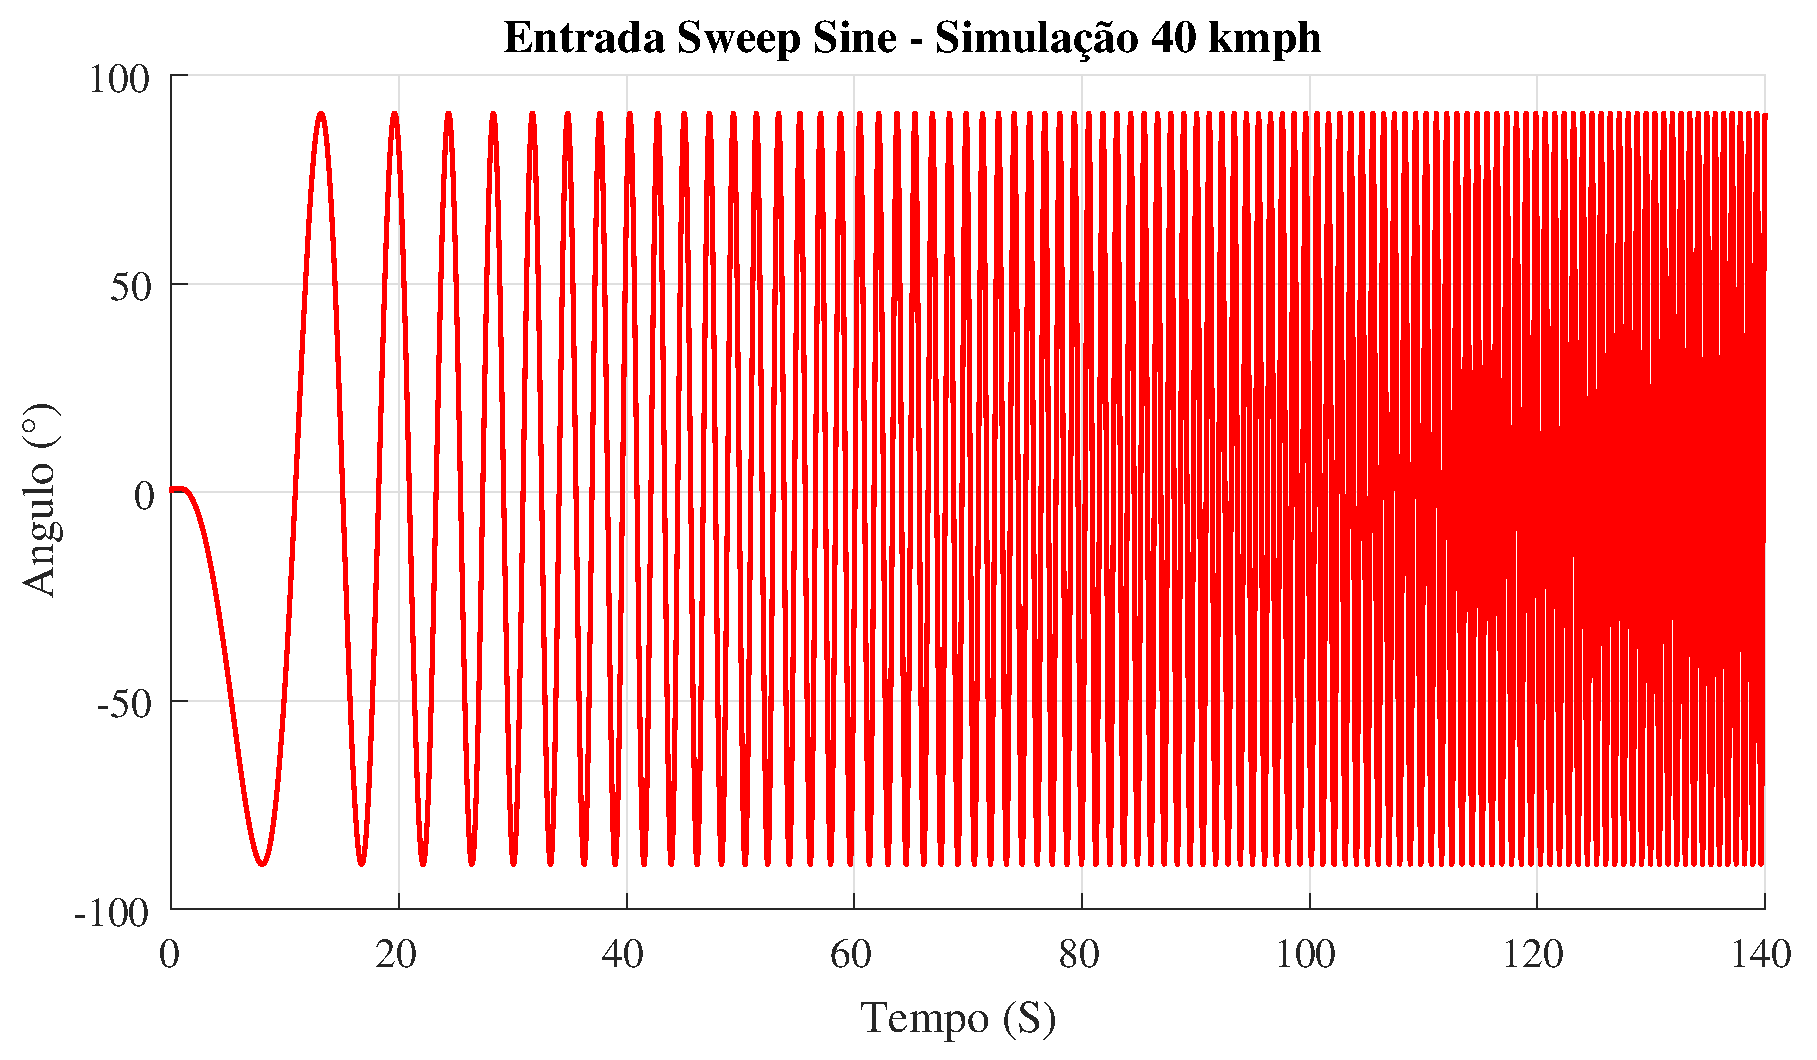
\includegraphics[width=10cm]{imagens/sweep40.eps}
\caption{Sinal de entrada: \textit{Sweep Sine}}
\label{fig:entrada40}
\end{figure}

Os resultados de cada um dos testes dada a simulação a 40 km/h são mostrados nas FIG. \ref{fig:saidaAcMin40}, \ref{fig:saidaVelMin40}, \ref{fig:saidaAccMax40} e \ref{fig:saidaVelMax40}.

\begin{figure}[H]
\centering
\subfigure[Aceleração lateral a uma entrada \textit{Sweep sine} a 40 km/h em carga mínima 
\label{fig:saidaAcMin40}]
{
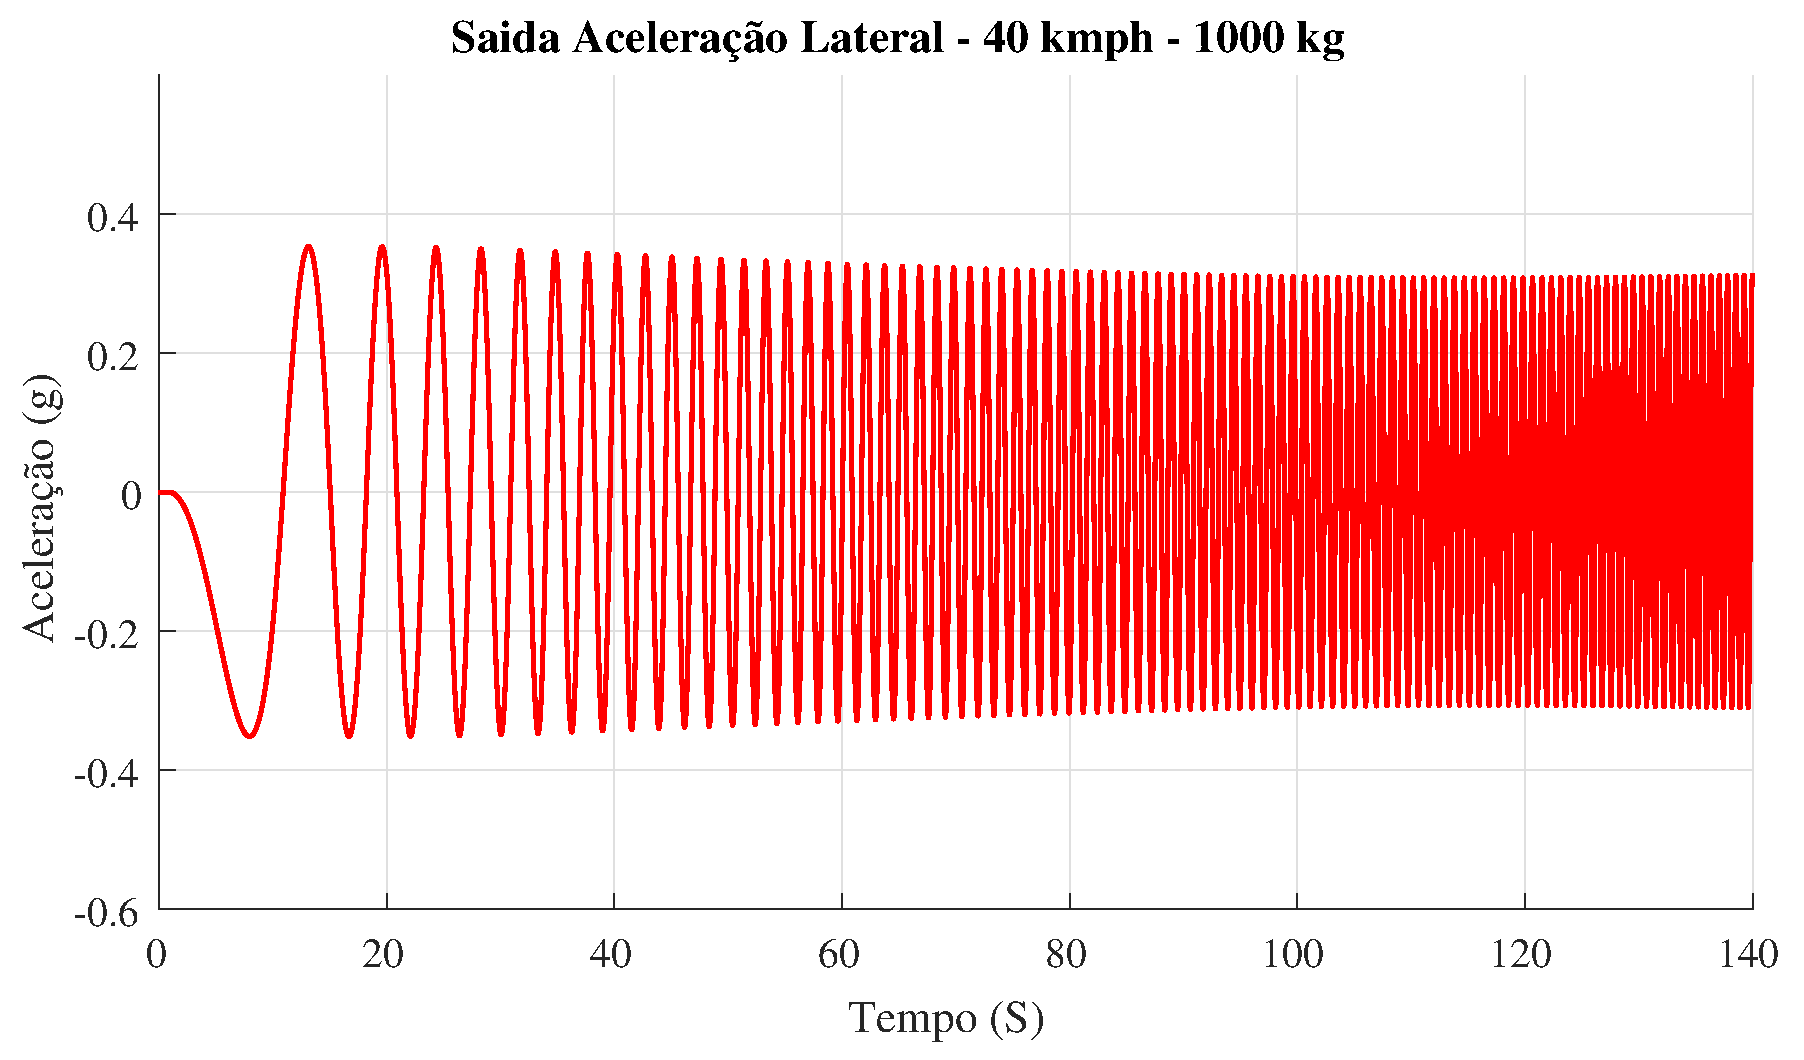
\includegraphics[width=7.5cm]{imagens/acc40min.eps}
}
\subfigure[Velocidade rotacional a uma entrada \textit{Sweep sine} a 40 km/h em carga mínima \label{fig:saidaVelMin40}]
{
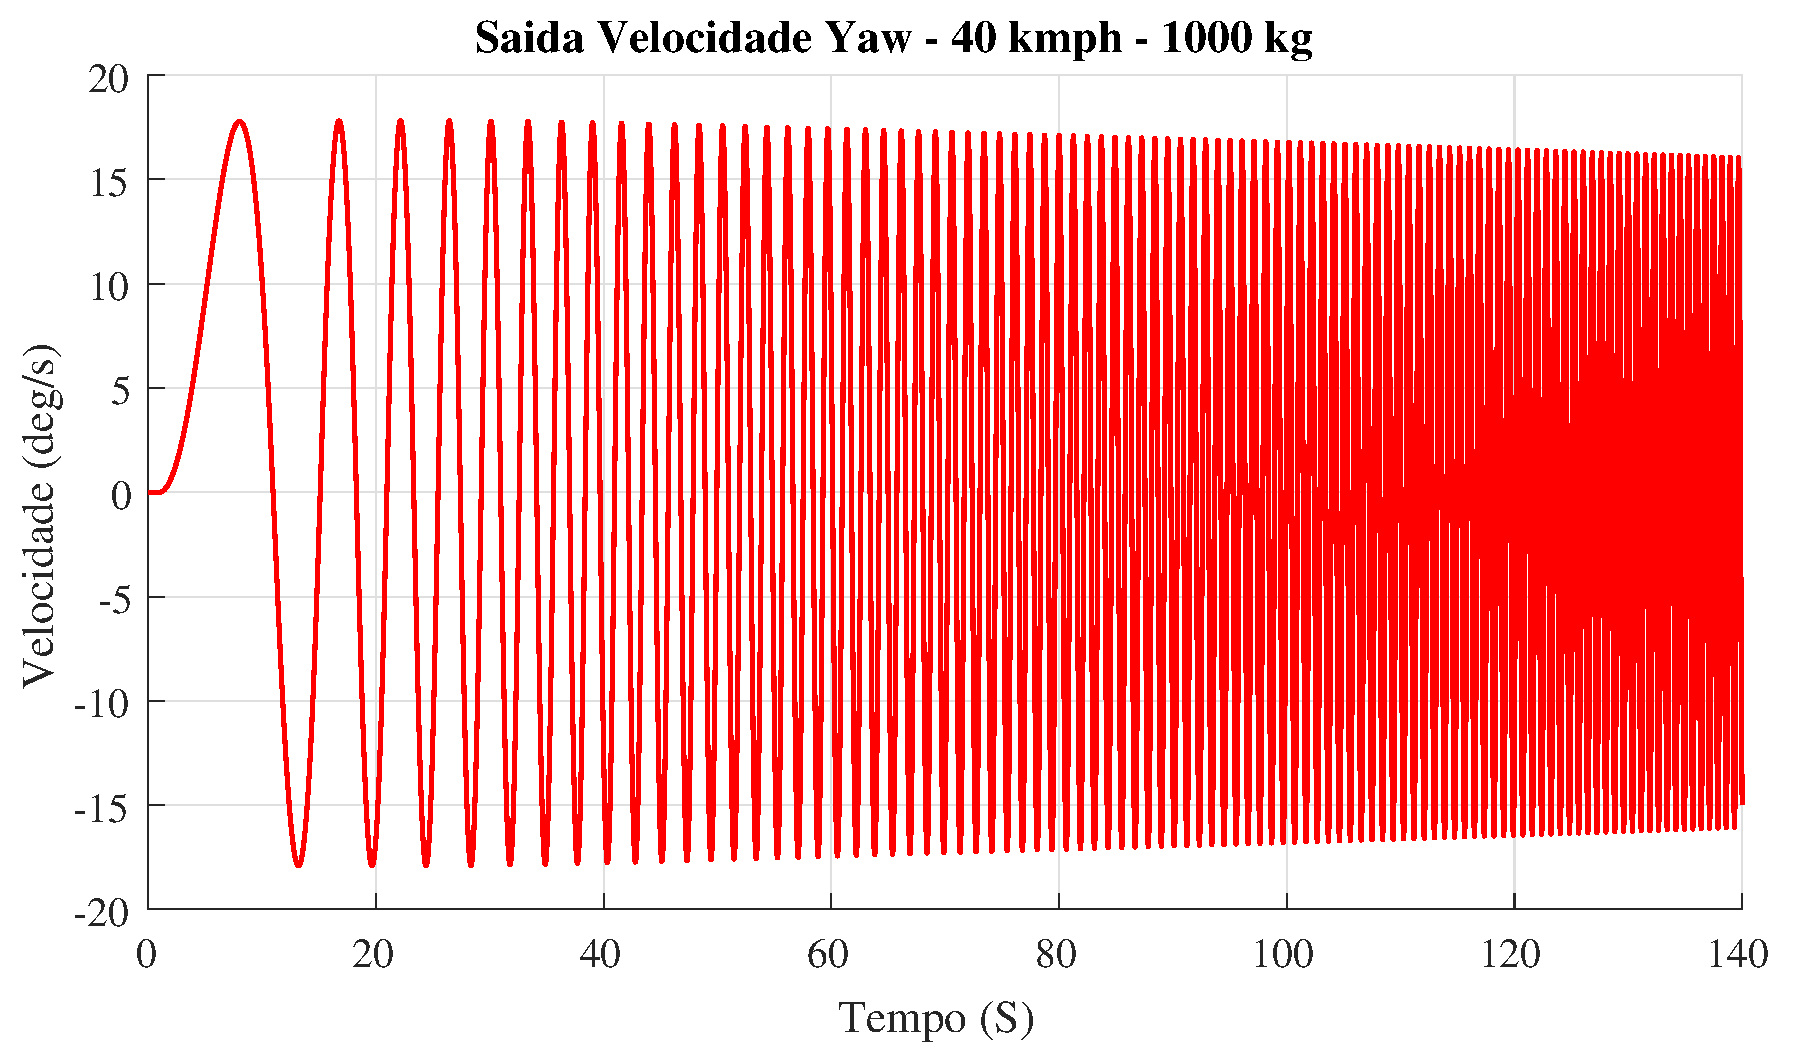
\includegraphics[width=7.5cm]{imagens/yaw40min.eps}
}
\subfigure[Aceleração lateral a uma entrada \textit{Sweep sine} a 40 km/h em carga máxima \label{fig:saidaAccMax40}]
{
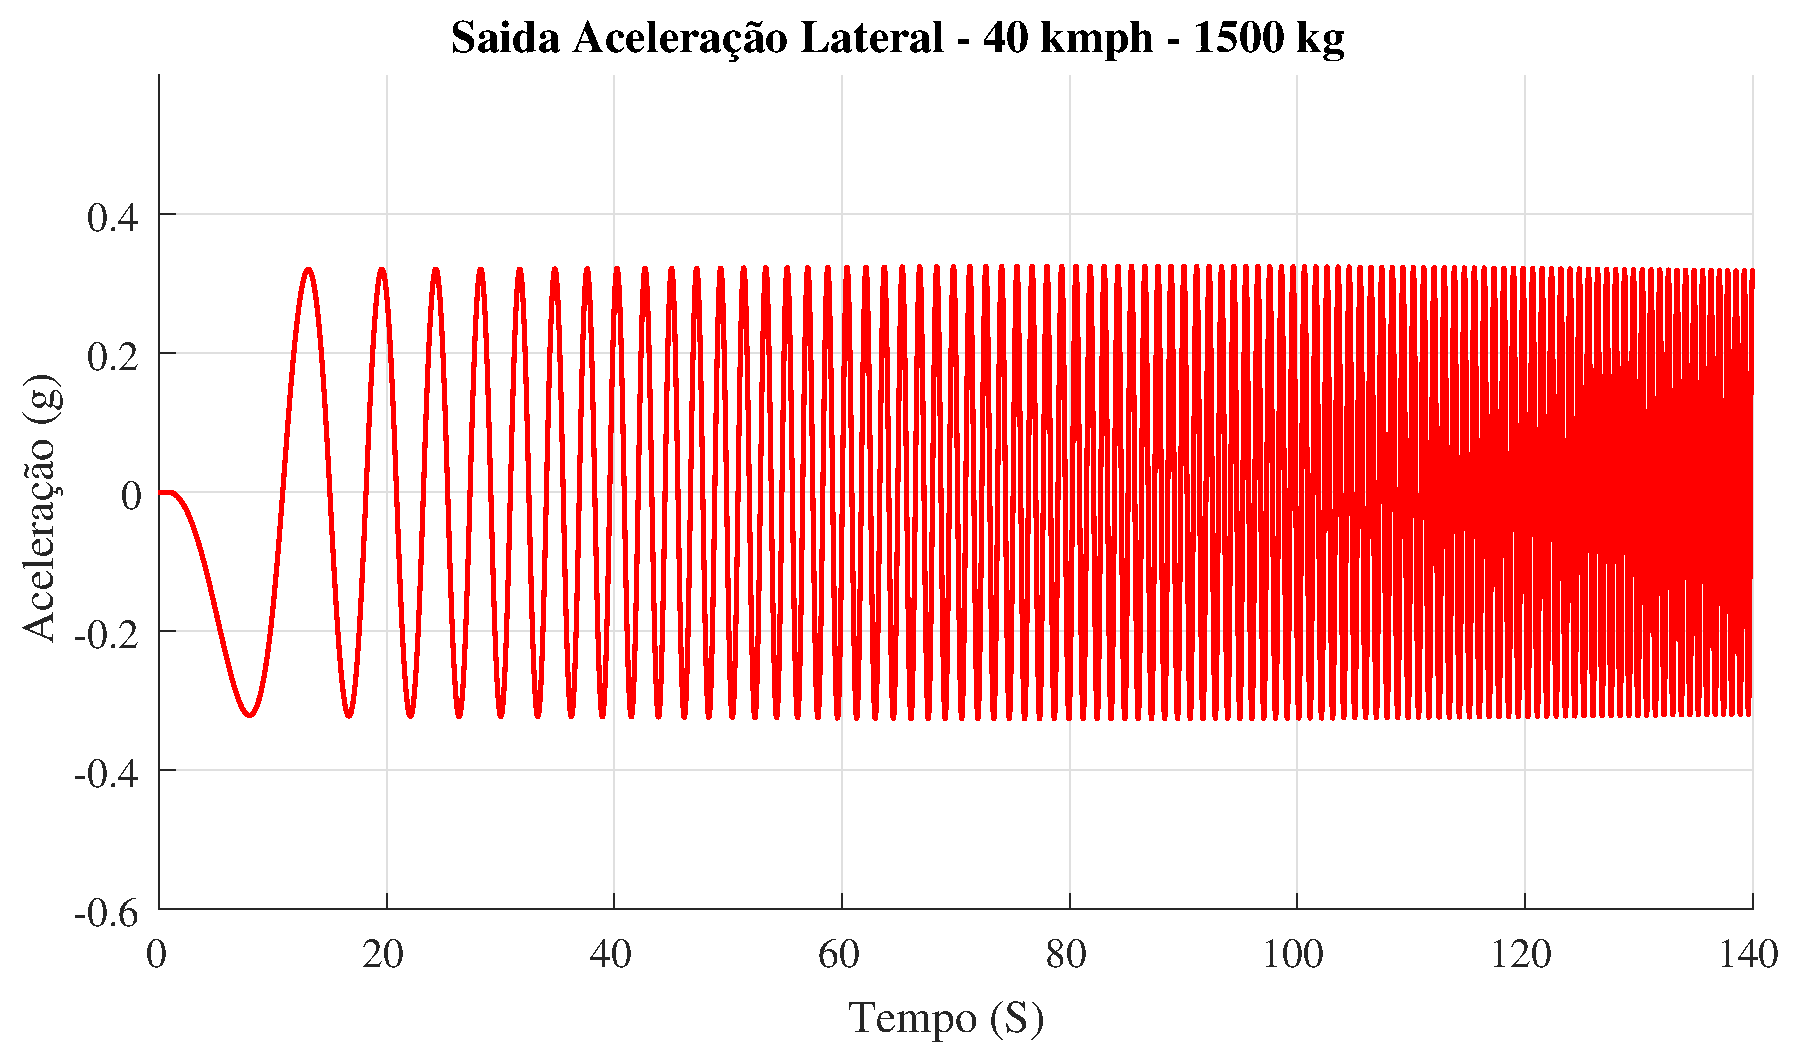
\includegraphics[width=7.5cm]{imagens/acc40max.eps}
}
\subfigure[Velocidade rotacional a uma entrada \textit{Sweep sine} a 40 km/h em carga máxima 
\label{fig:saidaVelMax40}]
{
\includegraphics[width=7.5cm]{imagens/yaw40max.eps}
}
\end{figure}


A curva de entrada para os testes a 100 km/h é dada pelo gráfico apresentado na FIG. \ref{fig:sweep_sine100}, cuja amplitude é de 15\si{\degree}, com frequência inicial de 0,001 Hz e final de 5 Hz.


\begin{figure}[H]
\centering
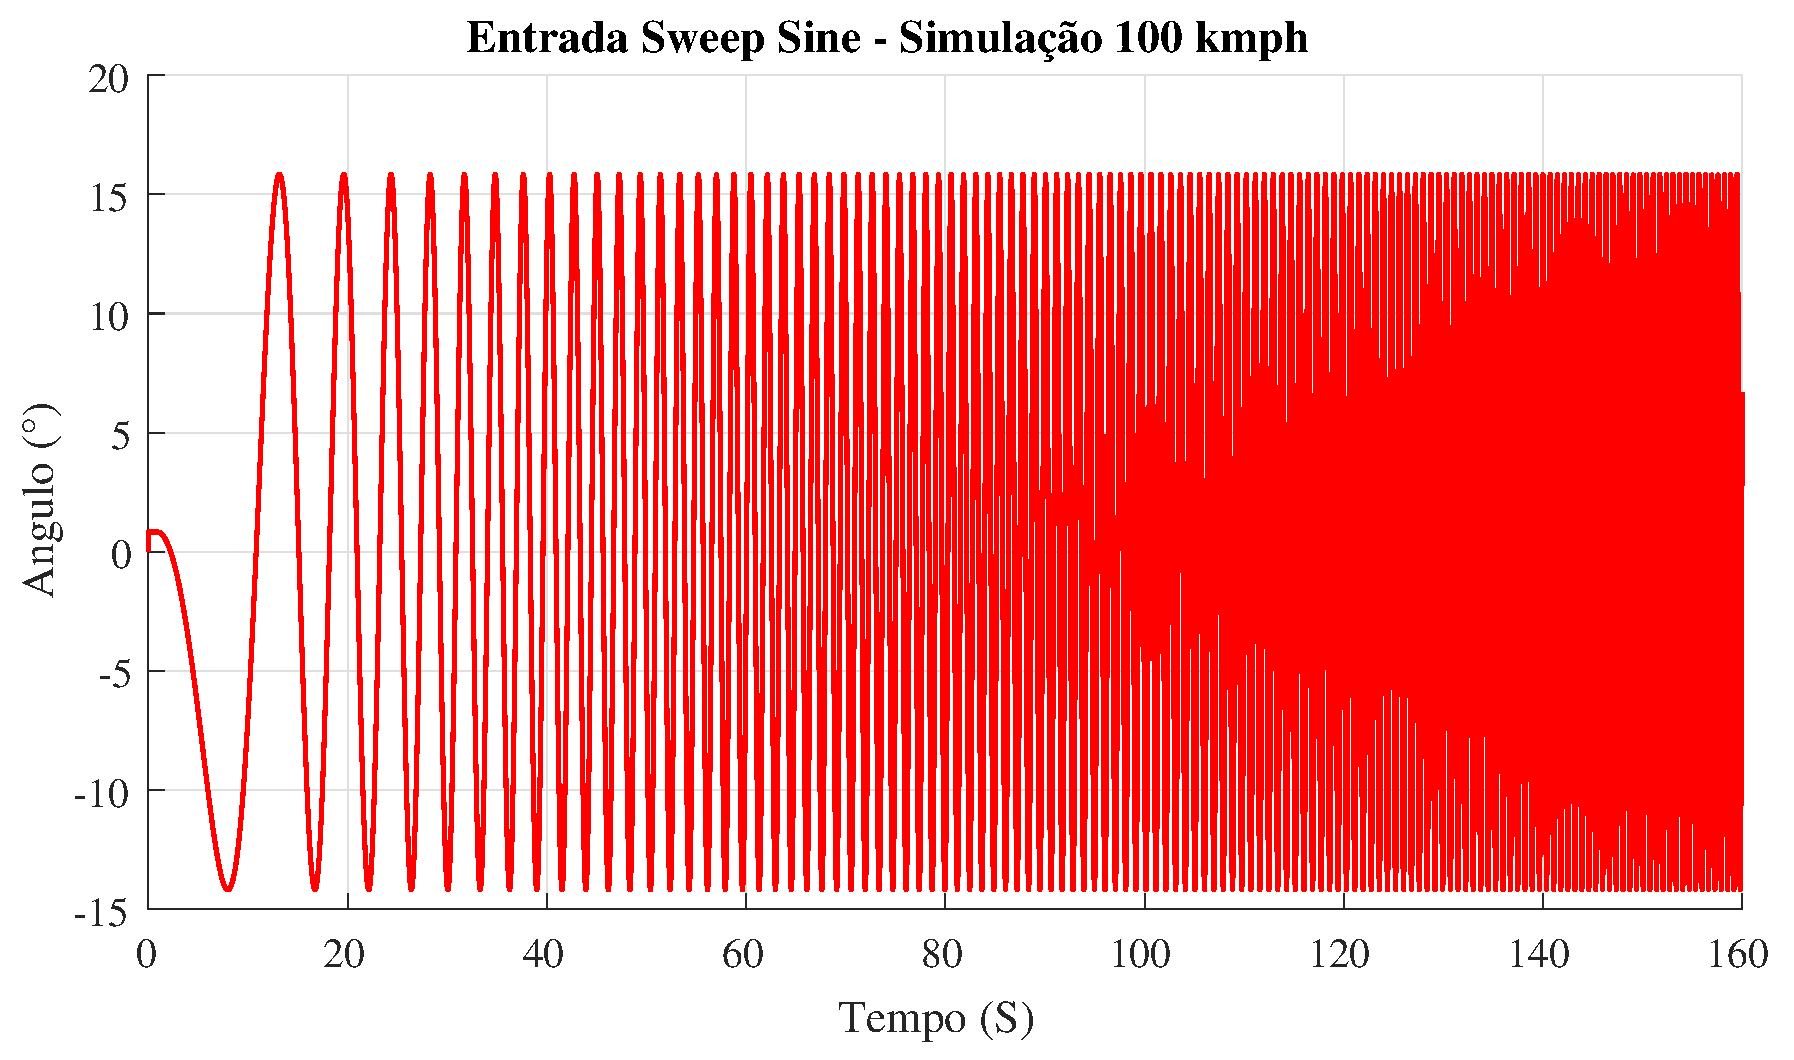
\includegraphics[width=10cm]{imagens/sweep100.eps}
\caption{Entrada \textit{Sweep Sine}, a 100 km/h}
\label{fig:sweep_sine100}
\end{figure}

E os resultados dos tetes para esta entrada são apresentados nas FIG. \ref{fig:saidaAcc100min}, \ref{fig:saidaVel100min}, \ref{fig:saidaAcc100Max} e \ref{fig:saidaVel100max}.

\begin{figure}[H]
\centering
\subfigure[Aceleração lateral a uma entrada \textit{Sweep sine} a 100 km/h em carga mínima \label{fig:saidaAcc100min}]
{
\includegraphics[width=7.5cm]{imagens/acc100min.eps}
}
\subfigure[Velocidade rotacional a uma entrada \textit{Sweep sine} a 100 km/h em carga mínima 
\label{fig:saidaVel100min}]
{
\includegraphics[width=7.5cm]{imagens/yaw100min.eps}
}
\subfigure[Aceleração lateral a uma entrada \textit{Sweep sine} a 100 km/h em carga máxima 
\label{fig:saidaAcc100Max}]
{
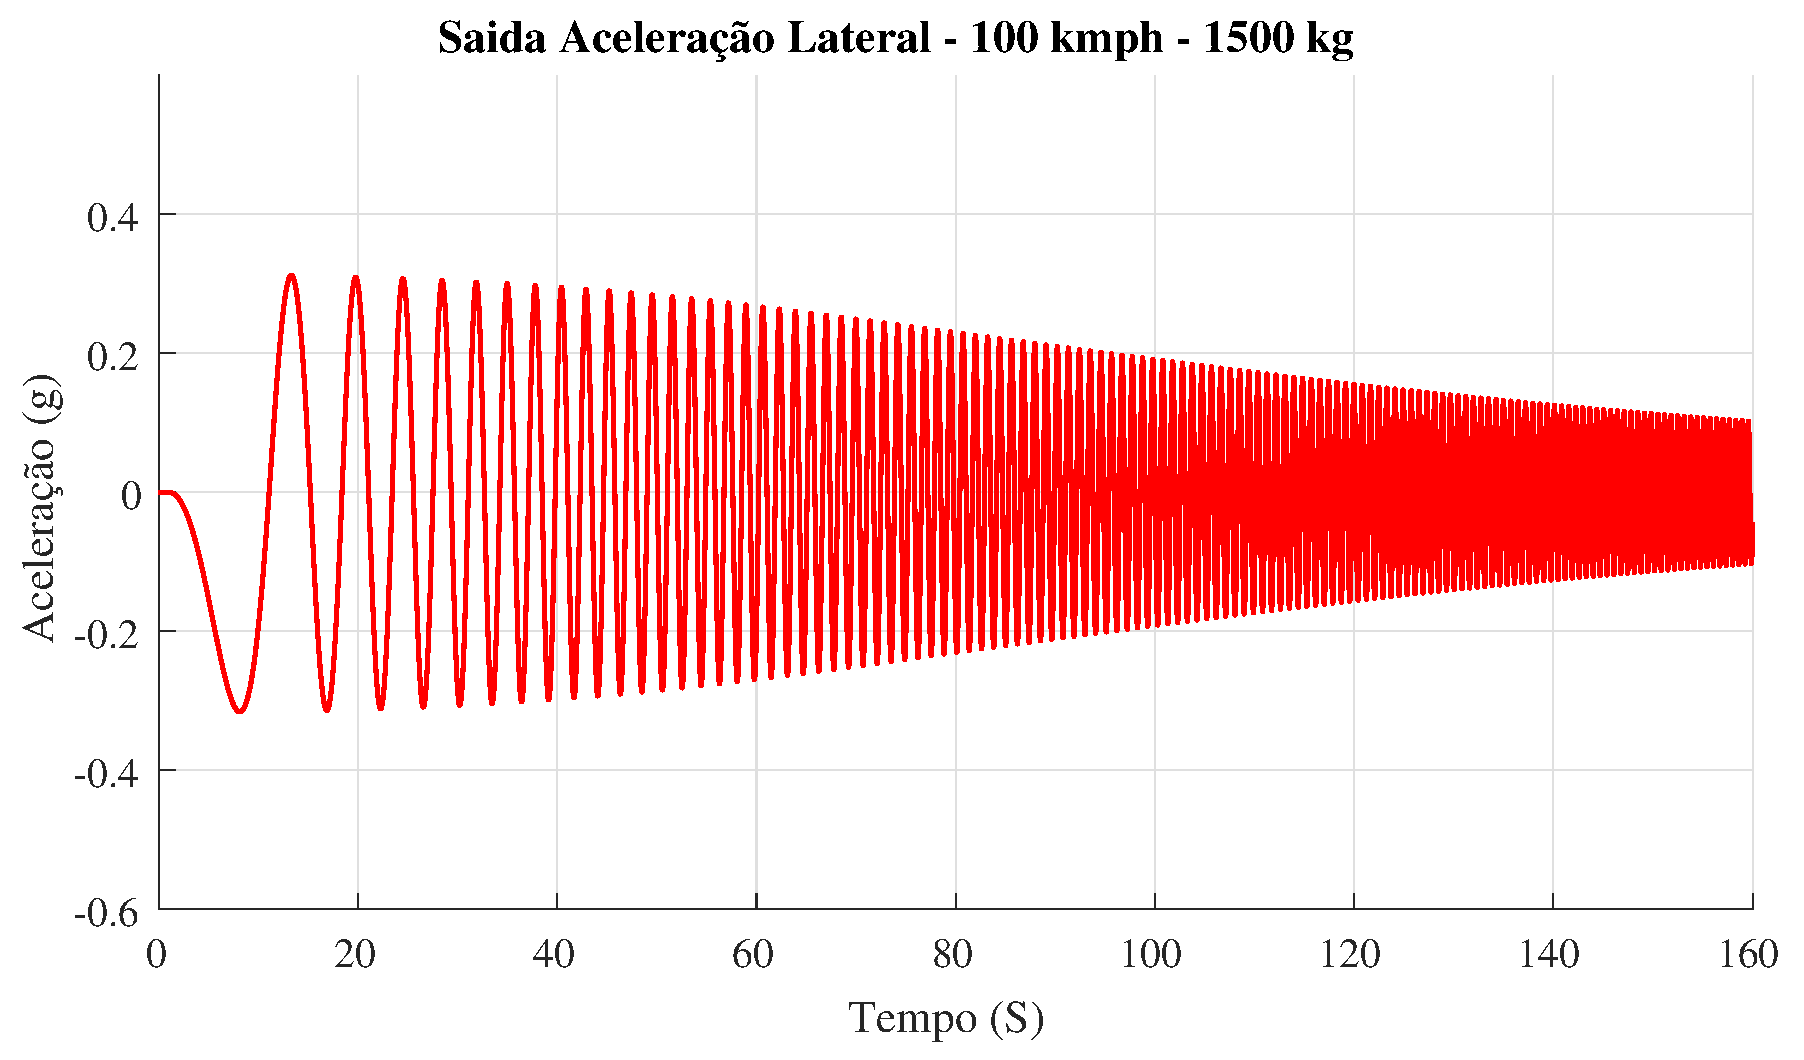
\includegraphics[width=7.5cm]{imagens/acc100max.eps}
}
\subfigure[Velocidade rotacional a uma entrada \textit{Sweep sine} a 100 km/h em carga máxima \label{fig:saidaVel100max}]
{
\includegraphics[width=7.5cm]{imagens/yaw100max.eps}
}
\end{figure}

Como é visto nos gráficos, as curvas apresentam o mesmo comportamento comparadas com as configurações similares de carga. Entretanto, percebe-se mais facilmente a deformação da amplitude a 100 km/h, embora o ângulo de entrada seja 6 vezes menor. Isto permite inferir que á medida que a velocidade aumenta, maior é sua influência na aceleração lateral. Tendendo a diminuir sua angulação significamente quando cresce a frequência de excitação.

Para a velocidade, é quase imperceptível, no domínio do tempo, as distorções que ocorrem na resposta. Com carga mínima pode-se afirmar asseguradamente que a amplitude diminui quando aumentado a frequência. Conquanto para a carga máxima se observa certa constância. Caso fosse traçado uma reta unindo os picos de cada senoide, ter-se-ia uma curva com um ponto de inflexão. Assinalando que em certa faixa a amplitude aumenta com a frequência e outra tem efeito oposto.

Faz-se as curvas comparativas a partir do diagrama de bode, que relaciona cada saída a sua respectiva entrada no domínio da frequência.
Uma comparação importante de ser feita é da resposta do veículo com carga miníma e máxima. Abaixo os diagramas fazem essa comparação:

\begin{figure}[H]
\centering
\includegraphics[width=13cm]{imagens/acc40.eps}
\caption{Diagrama de Bode da curvas \ref{fig:saidaAcMin40} e \ref{fig:saidaAccMax40}}
\label{graf:sweep_sine}
\end{figure}
\begin{figure}[H]
\centering
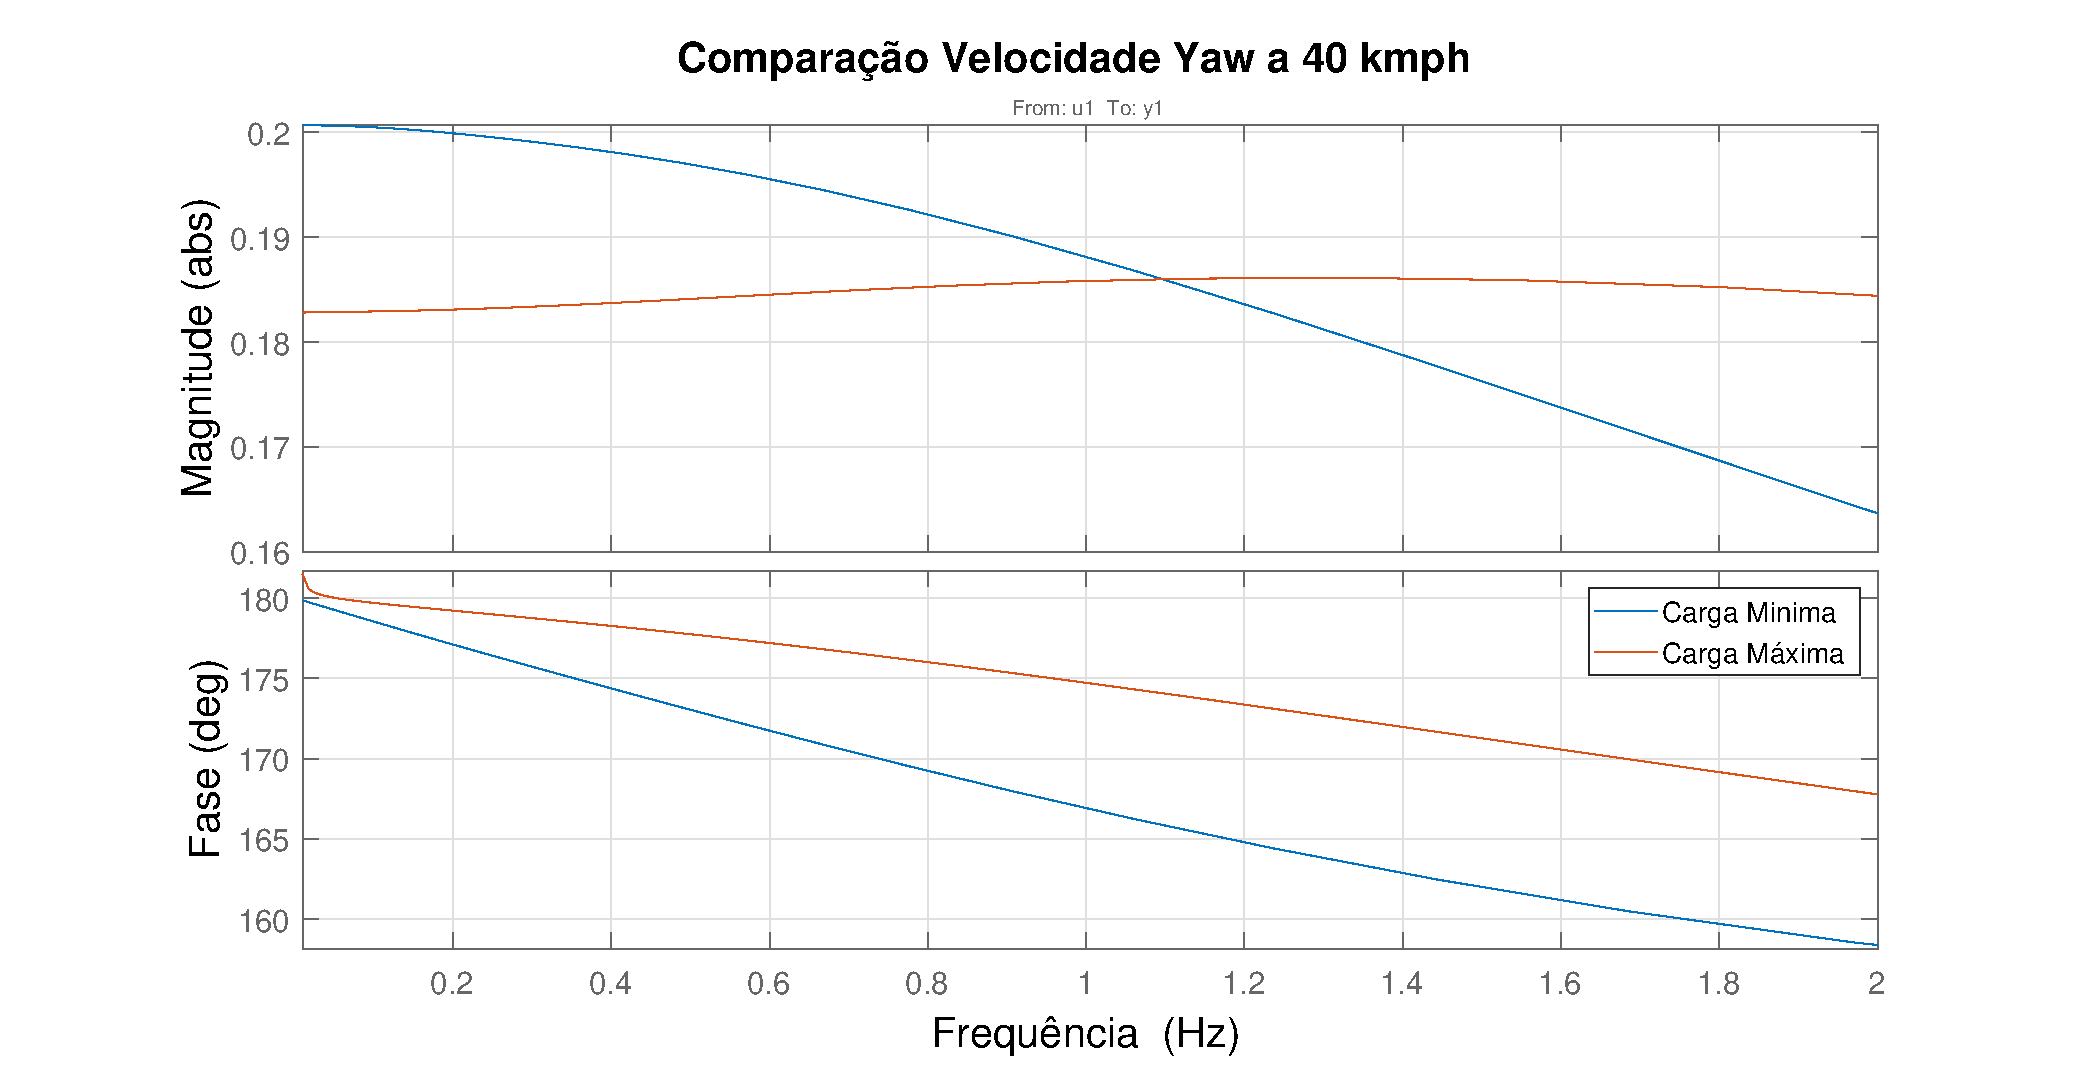
\includegraphics[width=13cm]{imagens/yaw40.eps}
\caption{Diagrama de Bode da curvas \ref{fig:saidaVelMin40} e \ref{fig:saidaVelMax40}}
\label{graf:sweep_sine}
\end{figure}
\begin{figure}[H]
\centering
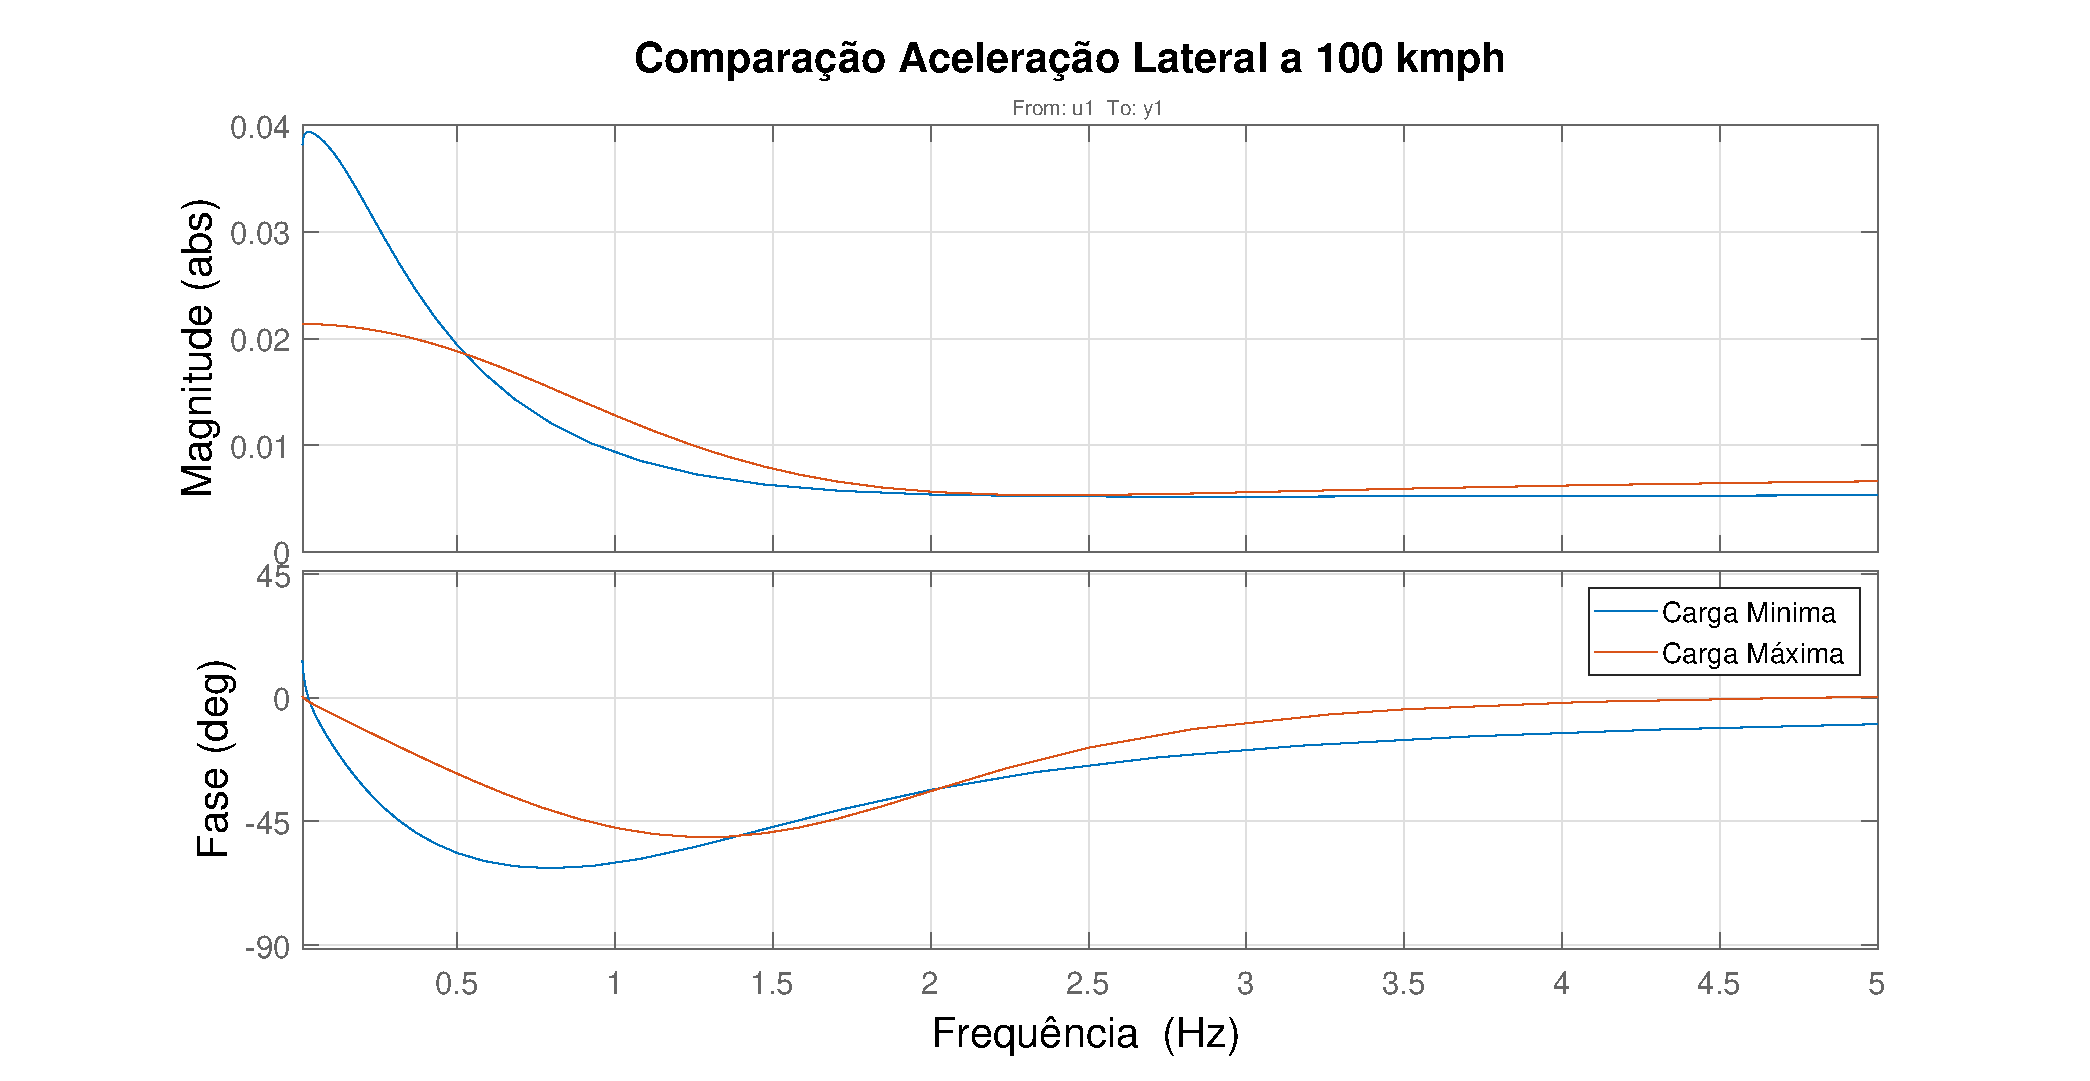
\includegraphics[width=13cm]{imagens/acc100.eps}
\caption{Diagrama de Bode da curvas \ref{fig:saidaAcc100min} e \ref{fig:saidaAcc100Max}}
\label{graf:sweep_sine}
\end{figure}
\begin{figure}[H]
\centering
\includegraphics[width=13cm]{imagens/yaw100.eps}
\caption{Diagrama de Bode da curvas \ref{fig:saidaVel100min} e \ref{fig:saidaVel100max}}
\label{graf:sweep_sine}
\end{figure}



\section{Conclusão}

Analisando as comparações no domínio da frequência, é possível perceber que o veículo se comporta de forma mais estável em carga máxima do que com carga mínima. Essa conclusão pode ser tirada dos diagramas de magnitude, onde com carga máxima a magnitude da aceleração lateral e a velocidade \textit{yaw} variam menos.


\section{Referências}
{\noindent
International Organization for Standardization. ISO 7401: Road Vehicles --- Lateral transient response test methods --- Open-loop test methods. Genebra, 2011. 
Disponível em: $<$ \url{https://www.sis.se/api/document/preview/913254/}$>$ Acesso em: 20 de Novembro de 2019.\vspace{0.5cm}
\\
PESCE et al., Handlig Quality Objective Evaluation of Light Commercial Vehicles. 2008. 30 slides. Disponível em: $<$\url{https://www.ukintpress-conferences.com/conf/08vdx_conf/pdf/day_1/marcopesce.pdf}$>$ Acesso em: 20 de Novembro de 2019. \vspace{0.5cm}
    \\
    KARLSSON A., Test Procedures and Evaluation Tools for Passenger Vehicle Dynamics: Master’s thesis in Automotive Engineering. Chalmers University of Thechnology: Department of Applied Mechanics Division of Vehicle Engineering and Autonomous Systems Vehicle Dynamics Group, Gotemburgo, 2014. Disponível em: $<$\url{http://publications.lib.chalmers.se/records/fulltext/211557/211557.pdf}$>$ Acesso em: 20 de Novembro de 2019.
    }
\end{document}
